% Options for packages loaded elsewhere
\PassOptionsToPackage{unicode}{hyperref}
\PassOptionsToPackage{hyphens}{url}
%
\documentclass[
]{article}
\usepackage{amsmath,amssymb}
\usepackage{lmodern}
\usepackage{iftex}
\ifPDFTeX
  \usepackage[T1]{fontenc}
  \usepackage[utf8]{inputenc}
  \usepackage{textcomp} % provide euro and other symbols
\else % if luatex or xetex
  \usepackage{unicode-math}
  \defaultfontfeatures{Scale=MatchLowercase}
  \defaultfontfeatures[\rmfamily]{Ligatures=TeX,Scale=1}
\fi
% Use upquote if available, for straight quotes in verbatim environments
\IfFileExists{upquote.sty}{\usepackage{upquote}}{}
\IfFileExists{microtype.sty}{% use microtype if available
  \usepackage[]{microtype}
  \UseMicrotypeSet[protrusion]{basicmath} % disable protrusion for tt fonts
}{}
\makeatletter
\@ifundefined{KOMAClassName}{% if non-KOMA class
  \IfFileExists{parskip.sty}{%
    \usepackage{parskip}
  }{% else
    \setlength{\parindent}{0pt}
    \setlength{\parskip}{6pt plus 2pt minus 1pt}}
}{% if KOMA class
  \KOMAoptions{parskip=half}}
\makeatother
\usepackage{xcolor}
\usepackage[margin=1in]{geometry}
\usepackage{longtable,booktabs,array}
\usepackage{calc} % for calculating minipage widths
% Correct order of tables after \paragraph or \subparagraph
\usepackage{etoolbox}
\makeatletter
\patchcmd\longtable{\par}{\if@noskipsec\mbox{}\fi\par}{}{}
\makeatother
% Allow footnotes in longtable head/foot
\IfFileExists{footnotehyper.sty}{\usepackage{footnotehyper}}{\usepackage{footnote}}
\makesavenoteenv{longtable}
\usepackage{graphicx}
\makeatletter
\def\maxwidth{\ifdim\Gin@nat@width>\linewidth\linewidth\else\Gin@nat@width\fi}
\def\maxheight{\ifdim\Gin@nat@height>\textheight\textheight\else\Gin@nat@height\fi}
\makeatother
% Scale images if necessary, so that they will not overflow the page
% margins by default, and it is still possible to overwrite the defaults
% using explicit options in \includegraphics[width, height, ...]{}
\setkeys{Gin}{width=\maxwidth,height=\maxheight,keepaspectratio}
% Set default figure placement to htbp
\makeatletter
\def\fps@figure{htbp}
\makeatother
\setlength{\emergencystretch}{3em} % prevent overfull lines
\providecommand{\tightlist}{%
  \setlength{\itemsep}{0pt}\setlength{\parskip}{0pt}}
\setcounter{secnumdepth}{5}
\usepackage{caption} \captionsetup{font={footnotesize},width=6in} \renewcommand{\dblfloatpagefraction}{.9} \makeatletter \renewenvironment{figure} {\def\@captype{figure}} \makeatletter \definecolor{shadecolor}{RGB}{242,242,242} \usepackage{xeCJK} \usepackage{setspace} \setstretch{1.3}
\ifLuaTeX
  \usepackage{selnolig}  % disable illegal ligatures
\fi
\IfFileExists{bookmark.sty}{\usepackage{bookmark}}{\usepackage{hyperref}}
\IfFileExists{xurl.sty}{\usepackage{xurl}}{} % add URL line breaks if available
\urlstyle{same} % disable monospaced font for URLs
\hypersetup{
  pdftitle={Report of Analysis},
  hidelinks,
  pdfcreator={LaTeX via pandoc}}

\title{Report of Analysis}
\author{}
\date{\vspace{-2.5em}}

\begin{document}
\maketitle

{
\setcounter{tocdepth}{3}
\tableofcontents
}
\hypertarget{ux7b2cux4e00ux90e8ux5206}{%
\section{第一部分}\label{ux7b2cux4e00ux90e8ux5206}}

\hypertarget{etcm-ux4e2dux836fux4e39ux53c2ux7684ux5316ux5408ux7269ux4ee5ux53caux9776ux70b9ux57faux56e0}{%
\subsection{ETCM 中药丹参的化合物以及靶点基因}\label{etcm-ux4e2dux836fux4e39ux53c2ux7684ux5316ux5408ux7269ux4ee5ux53caux9776ux70b9ux57faux56e0}}

丹参,ETCM ID 为73

丹参的96种化合物和相关靶基因概览
(对应文件为\texttt{./components\_and\_target\_genes.csv}):

\begin{verbatim}
## # A tibble: 532 x 3
##    components               genes  links                                                   
##    <chr>                    <chr>  <chr>                                                   
##  1 Sitosterol,Î’-Sitosterol AKR1C1 /ETCM/index.php/Home/Index/jyjb_details.html?gene=AKR1C1
##  2 Sitosterol,Î’-Sitosterol AKR1C2 /ETCM/index.php/Home/Index/jyjb_details.html?gene=AKR1C2
##  3 Sitosterol,Î’-Sitosterol AR     /ETCM/index.php/Home/Index/jyjb_details.html?gene=AR    
##  4 Sitosterol,Î’-Sitosterol CLEC4E /ETCM/index.php/Home/Index/jyjb_details.html?gene=CLEC4E
##  5 Sitosterol,Î’-Sitosterol ESR1   /ETCM/index.php/Home/Index/jyjb_details.html?gene=ESR1  
##  6 Sitosterol,Î’-Sitosterol ESR2   /ETCM/index.php/Home/Index/jyjb_details.html?gene=ESR2  
##  7 Sitosterol,Î’-Sitosterol GABRA1 /ETCM/index.php/Home/Index/jyjb_details.html?gene=GABRA1
##  8 Sitosterol,Î’-Sitosterol GABRA2 /ETCM/index.php/Home/Index/jyjb_details.html?gene=GABRA2
##  9 Sitosterol,Î’-Sitosterol GABRA3 /ETCM/index.php/Home/Index/jyjb_details.html?gene=GABRA3
## 10 Sitosterol,Î’-Sitosterol GABRA4 /ETCM/index.php/Home/Index/jyjb_details.html?gene=GABRA4
## # i 522 more rows
\end{verbatim}

\hypertarget{ux7b2cux4e8cux90e8ux5206}{%
\section{第二部分}\label{ux7b2cux4e8cux90e8ux5206}}

\hypertarget{ux5728genecardsux7f51ux7ad9ux4e0aux68c0ux7d22ux80c3ux764cux76f8ux5173ux7684ux57faux56e0}{%
\subsection{在genecards网站上检索胃癌相关的基因}\label{ux5728genecardsux7f51ux7ad9ux4e0aux68c0ux7d22ux80c3ux764cux76f8ux5173ux7684ux57faux56e0}}

根据Relevance score进行筛选(\textgreater{} 5)。
根据丹参靶点基因过滤数据集。

所有胃癌相关基因概览
(对应文件为\texttt{all\_gastric\_Cancer\_related\_genes.csv}):

\begin{verbatim}
## # A tibble: 4,475 x 8
##    Gene.Symbol Description           Category Uniprot.ID Gifts GC.Id Relevance.score GeneCards.Link
##    <chr>       <chr>                 <chr>    <chr>      <int> <chr>           <dbl> <chr>         
##  1 CDH1        Cadherin 1            Protein~ P12830        56 GC16~            379. https://www.g~
##  2 BRCA2       BRCA2 DNA Repair Ass~ Protein~ P51587        54 GC13~            303. https://www.g~
##  3 BRCA1       BRCA1 DNA Repair Ass~ Protein~ P38398        57 GC17~            291. https://www.g~
##  4 TP53        Tumor Protein P53     Protein~ P04637        60 GC17~            233. https://www.g~
##  5 APC         APC Regulator Of WNT~ Protein~ P25054        56 GC05~            218. https://www.g~
##  6 CHEK2       Checkpoint Kinase 2   Protein~ O96017        61 GC22~            204. https://www.g~
##  7 PALB2       Partner And Localize~ Protein~ Q86YC2        51 GC16~            204. https://www.g~
##  8 ATM         ATM Serine/Threonine~ Protein~ Q13315        60 GC11~            191. https://www.g~
##  9 MLH1        MutL Homolog 1        Protein~ P40692        56 GC03~            182. https://www.g~
## 10 BRIP1       BRCA1 Interacting He~ Protein~ Q9BX63        56 GC17~            180. https://www.g~
## # i 4,465 more rows
\end{verbatim}

韦恩图见图\ref{fig:fig2}
对应文件为\texttt{figs/venn\_plot.pdf}:

\begin{figure}
\centering
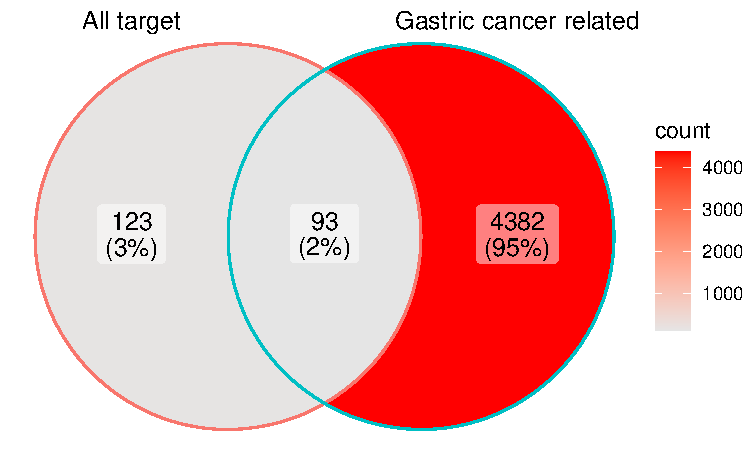
\includegraphics{figs/venn_plot.pdf}
\caption{\label{fig:fig2}靶点基因和胃癌相关基因交集韦恩图}
\end{figure}

96个化合物和胃癌相关基因的交集数据概览(包含交集基因以及对应化合物)
(对应文件为\texttt{gastric\_Cancer\_related\_genes\_Intersect\_with\_targetGenes\_components.csv}):

\begin{verbatim}
## # A tibble: 252 x 9
##    components               Gene.Symbol Description Category Uniprot.ID Gifts GC.Id Relevance.score
##    <chr>                    <chr>       <chr>       <chr>    <chr>      <int> <chr>           <dbl>
##  1 (25R)-5Α-Spirostan-3Β~ AR          Androgen R~ Protein~ P10275        58 GC0X~           64.6 
##  2 2-Isopropyl-8-Methylphe~ BGLAP       Bone Gamma~ Protein~ P02818        46 GC01~           11.2 
##  3 2-Isopropyl-8-Methylphe~ F2          Coagulatio~ Protein~ P00734        57 GC11~           14.2 
##  4 2-Isopropyl-8-Methylphe~ NQO1        NAD(P)H Qu~ Protein~ P15559        54 GC16~           29.7 
##  5 2-Isopropyl-8-Methylphe~ NQO2        N-Ribosyld~ Protein~ P16083        52 GC06~           21.6 
##  6 2-Isopropyl-8-Methylphe~ PROS1       Protein S   Protein~ P07225        56 GC03~            8.44
##  7 3,4-Dihydroxybenzoic Ac~ LCN2        Lipocalin 2 Protein~ P80188        52 GC09~           16.4 
##  8 3,4-Dihydroxybenzoic Ac~ MIF         Macrophage~ Protein~ P14174        54 GC22~           17.3 
##  9 3-O-Acetyloleanolic Acid ALOX5       Arachidona~ Protein~ P09917        54 GC10~           16.9 
## 10 3-O-Acetyloleanolic Acid ANXA1       Annexin A1  Protein~ P04083        53 GC09~           20.0 
## # i 242 more rows
## # i 1 more variable: GeneCards.Link <chr>
\end{verbatim}

\hypertarget{ux7b2cux4e09ux90e8ux5206}{%
\section{第三部分}\label{ux7b2cux4e09ux90e8ux5206}}

\hypertarget{ux4f7fux7528cellminerux6570ux636eux5e93ux7684nci-60}{%
\subsection{使用CellMiner数据库的NCI-60\ldots{}}\label{ux4f7fux7528cellminerux6570ux636eux5e93ux7684nci-60}}

Cisplatin 活性数据:

\begin{verbatim}
## # A tibble: 1 x 61
##   `Drug name` `BR:MCF7` `BR:MDA-MB-231` `BR:HS 578T` `BR:BT-549` `BR:T-47D` `CNS:SF-268`
##   <chr>       <chr>     <chr>           <chr>        <chr>       <chr>      <chr>       
## 1 Cisplatin   0.26      -1.8            -0.56        -0.29       -1.32      1.42        
## # i 54 more variables: `CNS:SF-295` <chr>, `CNS:SF-539` <chr>, `CNS:SNB-19` <chr>,
## #   `CNS:SNB-75` <chr>, `CNS:U251` <chr>, `CO:COLO 205` <chr>, `CO:HCC-2998` <chr>,
## #   `CO:HCT-116` <chr>, `CO:HCT-15` <chr>, `CO:HT29` <chr>, `CO:KM12` <chr>, `CO:SW-620` <chr>,
## #   `LE:CCRF-CEM` <chr>, `LE:HL-60(TB)` <chr>, `LE:K-562` <chr>, `LE:MOLT-4` <chr>,
## #   `LE:RPMI-8226` <chr>, `LE:SR` <chr>, `ME:LOX IMVI` <chr>, `ME:MALME-3M` <chr>, `ME:M14` <chr>,
## #   `ME:SK-MEL-2` <chr>, `ME:SK-MEL-28` <chr>, `ME:SK-MEL-5` <chr>, `ME:UACC-257` <chr>,
## #   `ME:UACC-62` <chr>, `ME:MDA-MB-435` <chr>, `ME:MDA-N` <chr>, `LC:A549/ATCC` <chr>, ...
\end{verbatim}

NCI-60 表达数据:

\begin{verbatim}
## # A tibble: 92 x 67
##    `Gene name d` `Entrez gene id e` `Chromosome f` `Start f`   `End f` `Cytoband f` `BR:MCF7`
##    <chr>                      <dbl> <chr>              <dbl>     <dbl> <chr>            <dbl>
##  1 SDHB                        6390 1               17345224  17380665 1p36.1-p35       4.99 
##  2 JAK1                        3716 1               65298905  65432187 1p32.3-p31.3     2.28 
##  3 ATP1A1                       476 1              116915794 116947396 1p21             4.99 
##  4 HSD3B1                      3283 1              120049825 120057681 1p13.1           0    
##  5 BGLAP                        632 1              156211752 156213123 1q22             0.438
##  6 SDHC                        6391 1              161284165 161334535 1q23.3           2.55 
##  7 ESRRG                       2104 1              216676587 217311097 1q41             0    
##  8 CYP1B1                      1545 2               38294745  38303323 2p22.2           2.02 
##  9 IL1B                        3553 2              113587336 113594356 2q14             0    
## 10 PPARG                       5468 3               12329348  12475855 3p25             0.588
## # i 82 more rows
## # i 60 more variables: `BR:MDA-MB-231` <dbl>, `BR:HS 578T` <dbl>, `BR:BT-549` <dbl>,
## #   `BR:T-47D` <dbl>, `CNS:SF-268` <dbl>, `CNS:SF-295` <dbl>, `CNS:SF-539` <dbl>,
## #   `CNS:SNB-19` <dbl>, `CNS:SNB-75` <dbl>, `CNS:U251` <dbl>, `CO:COLO 205` <dbl>,
## #   `CO:HCC-2998` <dbl>, `CO:HCT-116` <dbl>, `CO:HCT-15` <dbl>, `CO:HT29` <dbl>, `CO:KM12` <dbl>,
## #   `CO:SW-620` <dbl>, `LE:CCRF-CEM` <dbl>, `LE:HL-60(TB)` <dbl>, `LE:K-562` <dbl>,
## #   `LE:MOLT-4` <dbl>, `LE:RPMI-8226` <dbl>, `LE:SR` <dbl>, `ME:LOX IMVI` <dbl>, ...
\end{verbatim}

\hypertarget{ux836fux7269ux654fux611fux6027ux5206ux6790}{%
\subsection{药物敏感性分析}\label{ux836fux7269ux654fux611fux6027ux5206ux6790}}

其中有显著性意义的有13个基因(所有化合物),可视化见图\ref{fig:fig3}
(对应文件为\texttt{figs/pearsonTest.pdf})

\begin{figure}
\centering
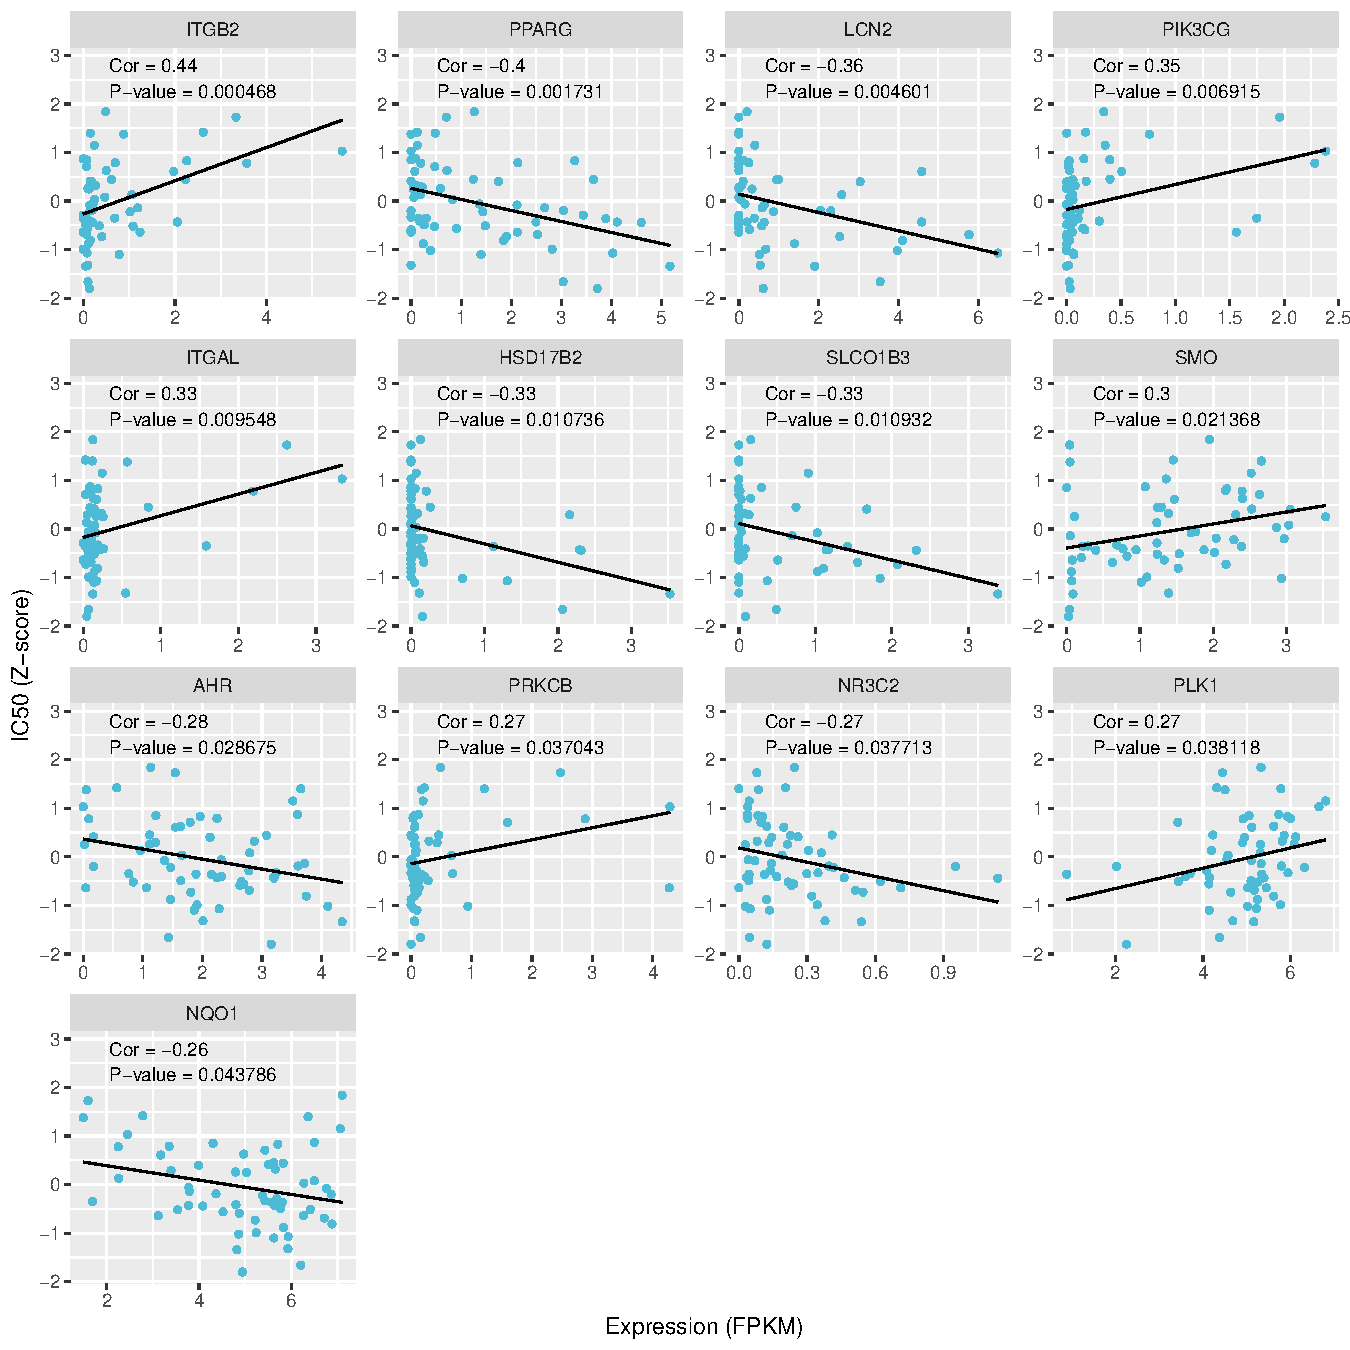
\includegraphics{figs/pearsonTest.pdf}
\caption{\label{fig:fig3}关联性分析回归曲线图}
\end{figure}

关联性分析(Pearson)结果概览(已包含基因和对应化合物数据)(对应文件为\texttt{./pearsonTest\_allResults.csv} 和 \texttt{./pearsonTest\_results\_with\_components.csv}):

\begin{verbatim}
## # A tibble: 28 x 11
##    name       cor  p.value components   Description Category Uniprot.ID Gifts GC.Id Relevance.score
##    <chr>    <dbl>    <dbl> <chr>        <chr>       <chr>    <chr>      <int> <chr>           <dbl>
##  1 AHR     -0.283 0.0287   Baicalin     Aryl Hydro~ Protein~ P35869        53 GC07~           14.6 
##  2 HSD17B2 -0.327 0.0107   Salviol      Hydroxyste~ Protein~ P37059        49 GC16~            8.14
##  3 ITGAL    0.332 0.00955  3-O-Acetylo~ Integrin S~ Protein~ P20701        53 GC16~            6.80
##  4 ITGAL    0.332 0.00955  Oleoyl Neoc~ Integrin S~ Protein~ P20701        53 GC16~            6.80
##  5 ITGB2    0.438 0.000468 Oleoyl Neoc~ Integrin S~ Protein~ P05107        57 GC21~            5.77
##  6 ITGB2    0.438 0.000468 3-O-Acetylo~ Integrin S~ Protein~ P05107        57 GC21~            5.77
##  7 LCN2    -0.361 0.00460  Protocatech~ Lipocalin 2 Protein~ P80188        52 GC09~           16.4 
##  8 LCN2    -0.361 0.00460  3,4-Dihydro~ Lipocalin 2 Protein~ P80188        52 GC09~           16.4 
##  9 NQO1    -0.261 0.0438   2-Isopropyl~ NAD(P)H Qu~ Protein~ P15559        54 GC16~           29.7 
## 10 NR3C2   -0.269 0.0377   Oleanolic A~ Nuclear Re~ Protein~ P08235        53 GC04~            7.79
## # i 18 more rows
## # i 1 more variable: GeneCards.Link <chr>
\end{verbatim}

\hypertarget{ux7b2cux56dbux90e8ux5206}{%
\section{第四部分}\label{ux7b2cux56dbux90e8ux5206}}

\hypertarget{ux4f7fux7528biomartux6ce8ux91caux9776ux70b9ux57faux56e0}{%
\subsection{使用BiomaRt注释靶点基因}\label{ux4f7fux7528biomartux6ce8ux91caux9776ux70b9ux57faux56e0}}

获取Entrezgene id 以便后续分析\ldots\ldots{}

\begin{verbatim}
## # A tibble: 13 x 3
##    ensembl_gene_id entrezgene_id hgnc_symbol
##    <chr>                   <int> <chr>      
##  1 ENSG00000106546           196 AHR        
##  2 ENSG00000086696          3294 HSD17B2    
##  3 ENSG00000005844          3683 ITGAL      
##  4 ENSG00000160255          3689 ITGB2      
##  5 ENSG00000148346          3934 LCN2       
##  6 ENSG00000181019          1728 NQO1       
##  7 ENSG00000151623          4306 NR3C2      
##  8 ENSG00000105851          5294 PIK3CG     
##  9 ENSG00000166851          5347 PLK1       
## 10 ENSG00000132170          5468 PPARG      
## 11 ENSG00000166501          5579 PRKCB      
## 12 ENSG00000111700         28234 SLCO1B3    
## 13 ENSG00000128602          6608 SMO
\end{verbatim}

将注释数据与筛选的化合物的靶点基因数据合并,并按照化合物分组。

各个化合物包含的显著性靶点基因数量信息:

\begin{verbatim}
## $`2-Isopropyl-8-Methylphenanthrene-3,4-Dione(R0-090680)`
## [1] 1
## 
## $`3-O-Acetyloleanolic Acid`
## [1] 3
## 
## $`3,4-Dihydroxybenzoic Acid,Protocatechuic Acid`
## [1] 1
## 
## $`Alexandrin,Daucosterol,Caproic Acid,Eleutheroside A,Sitogluside,Strumaroside,Î’-Sitosterol-Î’-D-Glucoside`
## [1] 1
## 
## $`Alexandrin,Daucosterol,Eleutheroside A`
## [1] 1
## 
## $Baicalin
## [1] 3
## 
## $`Danshenol B`
## [1] 1
## 
## $Ferruginol
## [1] 2
## 
## $Miltipolone
## [1] 1
## 
## $`Oleanolic Acid`
## [1] 1
## 
## $`Oleoyl Neocryptotanshinone`
## [1] 3
## 
## $`Protocatechuic Aldehyde`
## [1] 1
## 
## $`Rosmarinic Acid Methyl Ester`
## [1] 1
## 
## $Salviol
## [1] 2
## 
## $`Sitosterol,Î’-Sitosterol`
## [1] 1
## 
## $Stigmasterol
## [1] 1
## 
## $Sugiol
## [1] 1
## 
## $Tanshinaldehyde
## [1] 2
## 
## $`Ursolic Acid`
## [1] 1
\end{verbatim}

所有化合物都不包含超过5个靶点基因

\hypertarget{ux4f7fux7528clusterprofilerux5bccux96c6ux5206ux6790}{%
\subsection{\texorpdfstring{使用\texttt{clusterProfiler}富集分析}{使用clusterProfiler富集分析}}\label{ux4f7fux7528clusterprofilerux5bccux96c6ux5206ux6790}}

说明:KEGG富集分析都有结果;但是对于GO 富集分析(BP,CC 或 MF)中,个别化合物有靶点基因,但未映射到通路中的基因,所以无结果, 这些是(TRUE表示有结果,而FALSE表示无结果):

\begin{verbatim}
## $`2-Isopropyl-8-Methylphenanthrene-3,4-Dione(R0-090680)`
##   BP   CC   MF 
## TRUE TRUE TRUE 
## 
## $`3-O-Acetyloleanolic Acid`
##   BP   CC   MF 
## TRUE TRUE TRUE 
## 
## $`3,4-Dihydroxybenzoic Acid,Protocatechuic Acid`
##   BP   CC   MF 
## TRUE TRUE TRUE 
## 
## $`Alexandrin,Daucosterol,Caproic Acid,Eleutheroside A,Sitogluside,Strumaroside,Î’-Sitosterol-Î’-D-Glucoside`
##   BP   CC   MF 
## TRUE TRUE TRUE 
## 
## $`Alexandrin,Daucosterol,Eleutheroside A`
##   BP   CC   MF 
## TRUE TRUE TRUE 
## 
## $Baicalin
##   BP   CC   MF 
## TRUE TRUE TRUE 
## 
## $`Danshenol B`
##    BP    CC    MF 
##  TRUE  TRUE FALSE 
## 
## $Ferruginol
##   BP   CC   MF 
## TRUE TRUE TRUE 
## 
## $Miltipolone
##   BP   CC   MF 
## TRUE TRUE TRUE 
## 
## $`Oleanolic Acid`
##    BP    CC    MF 
##  TRUE FALSE  TRUE 
## 
## $`Oleoyl Neocryptotanshinone`
##   BP   CC   MF 
## TRUE TRUE TRUE 
## 
## $`Protocatechuic Aldehyde`
##   BP   CC   MF 
## TRUE TRUE TRUE 
## 
## $`Rosmarinic Acid Methyl Ester`
##   BP   CC   MF 
## TRUE TRUE TRUE 
## 
## $Salviol
##   BP   CC   MF 
## TRUE TRUE TRUE 
## 
## $`Sitosterol,Î’-Sitosterol`
##    BP    CC    MF 
##  TRUE FALSE  TRUE 
## 
## $Stigmasterol
##    BP    CC    MF 
##  TRUE FALSE  TRUE 
## 
## $Sugiol
##   BP   CC   MF 
## TRUE TRUE TRUE 
## 
## $Tanshinaldehyde
##   BP   CC   MF 
## TRUE TRUE TRUE 
## 
## $`Ursolic Acid`
##    BP    CC    MF 
##  TRUE FALSE  TRUE
\end{verbatim}

图片数量较多,不一一展示。
对应文件为:\texttt{./enrichGO} 或 \texttt{./enrichKEGG} 文件夹下图片

\end{document}
